\documentclass[10pt]{article}
\usepackage[polish]{babel}
\usepackage[utf8]{inputenc}
\usepackage[T1]{fontenc}
\usepackage{graphicx}
\usepackage[export]{adjustbox}
\graphicspath{ {./images/} }
\usepackage{amsmath}
\usepackage{amsfonts}
\usepackage{amssymb}
\usepackage[version=4]{mhchem}
\usepackage{stmaryrd}
\usepackage{multirow}

\title{EGZAMIN MATURALNY Z MATEMATYKI }

\author{Data:9 maja 2019 r.\\
Godzina rozpoczeclia: 9:00\\
CZAS PRACY: \(\mathbf{1 8 0}\) minut\\
LICZBA PUNKTÓW DO UZYSKANIA: \(\mathbf{5 0}\)}
\date{}


\begin{document}
\maketitle
\begin{center}
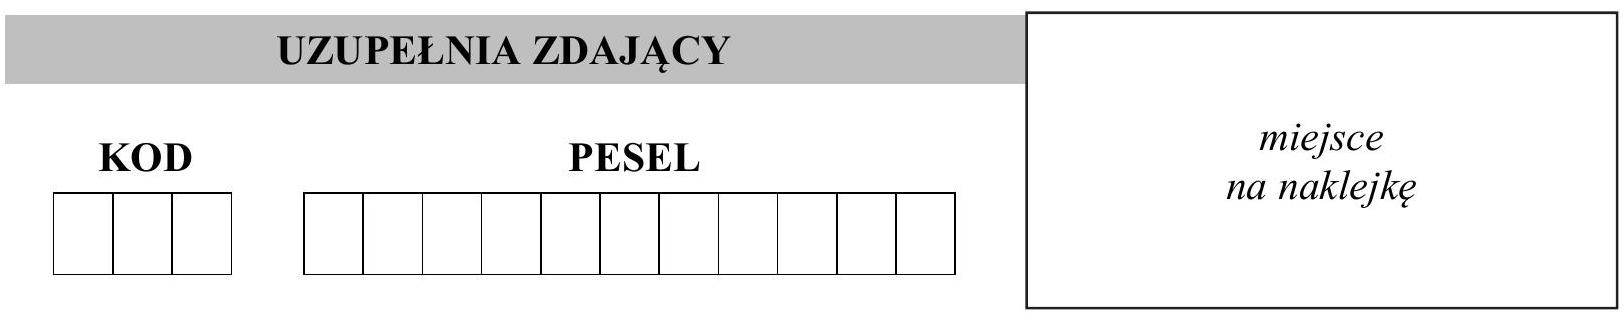
\includegraphics[max width=\textwidth]{2024_11_21_9df891ea1c7ef9791261g-01}
\end{center}

POZIOM ROZSZERZONY

\begin{center}
\begin{tabular}{|c|}
\hline
UZUPELNIA ZESPÓŁ \\
NADZORUJĄCY \\
\hline
Uprawnienia zdającego do: \\
\(\square \quad\)\begin{tabular}{l}
dostosowania \\
kryteriów oceniania \\
\(\square \quad\)\begin{tabular}{l}
nieprzenoszenia \\
zaznaczeń na karte \\
\end{tabular} \\
\hline
\end{tabular} \\
\hline
\end{tabular}
\end{center}

\section*{Instrukcja dla zdającego}
\begin{enumerate}
  \item Sprawdź, czy arkusz egzaminacyjny zawiera 22 strony (zadania 1-15).
\end{enumerate}

Ewentualny brak zgłoś przewodniczącemu zespołu nadzorującego egzamin.\\
2. Rozwiązania zadań i odpowiedzi wpisuj w miejscu na to przeznaczonym.\\
3. Odpowiedzi do zadań zamkniętych (1-4) zaznacz na karcie odpowiedzi w części karty przeznaczonej dla zdającego. Zamaluj \(\square\) pola do tego przeznaczone. Błędne zaznaczenie otocz kółkiem \()_{\text {i zaznacz właściwe. }}\)\\
4. W zadaniu 5. wpisz odpowiednie cyfry w kratki pod treścią zadania.\\
5. Pamiętaj, że pominięcie argumentacji lub istotnych obliczeń w rozwiązaniu zadania otwartego (6-15) może spowodować, że za to rozwiązanie nie otrzymasz pełnej liczby punktów.\\
6. Pisz czytelnie i używaj tylko długopisu lub pióra z czarnym tuszem lub atramentem.\\
7. Nie używaj korektora, a błędne zapisy wyraźnie przekreśl.\\
8. Pamiętaj, że zapisy w brudnopisie nie będą oceniane.\\
9. Możesz korzystać z zestawu wzorów matematycznych, cyrkla i linijki oraz kalkulatora prostego.\\
10. Na tej stronie oraz na karcie odpowiedzi wpisz swój numer PESEL i przyklej naklejkę z kodem.\\
11. Nie wpisuj żadnych znaków w części przeznaczonej dla egzaminatora.\\
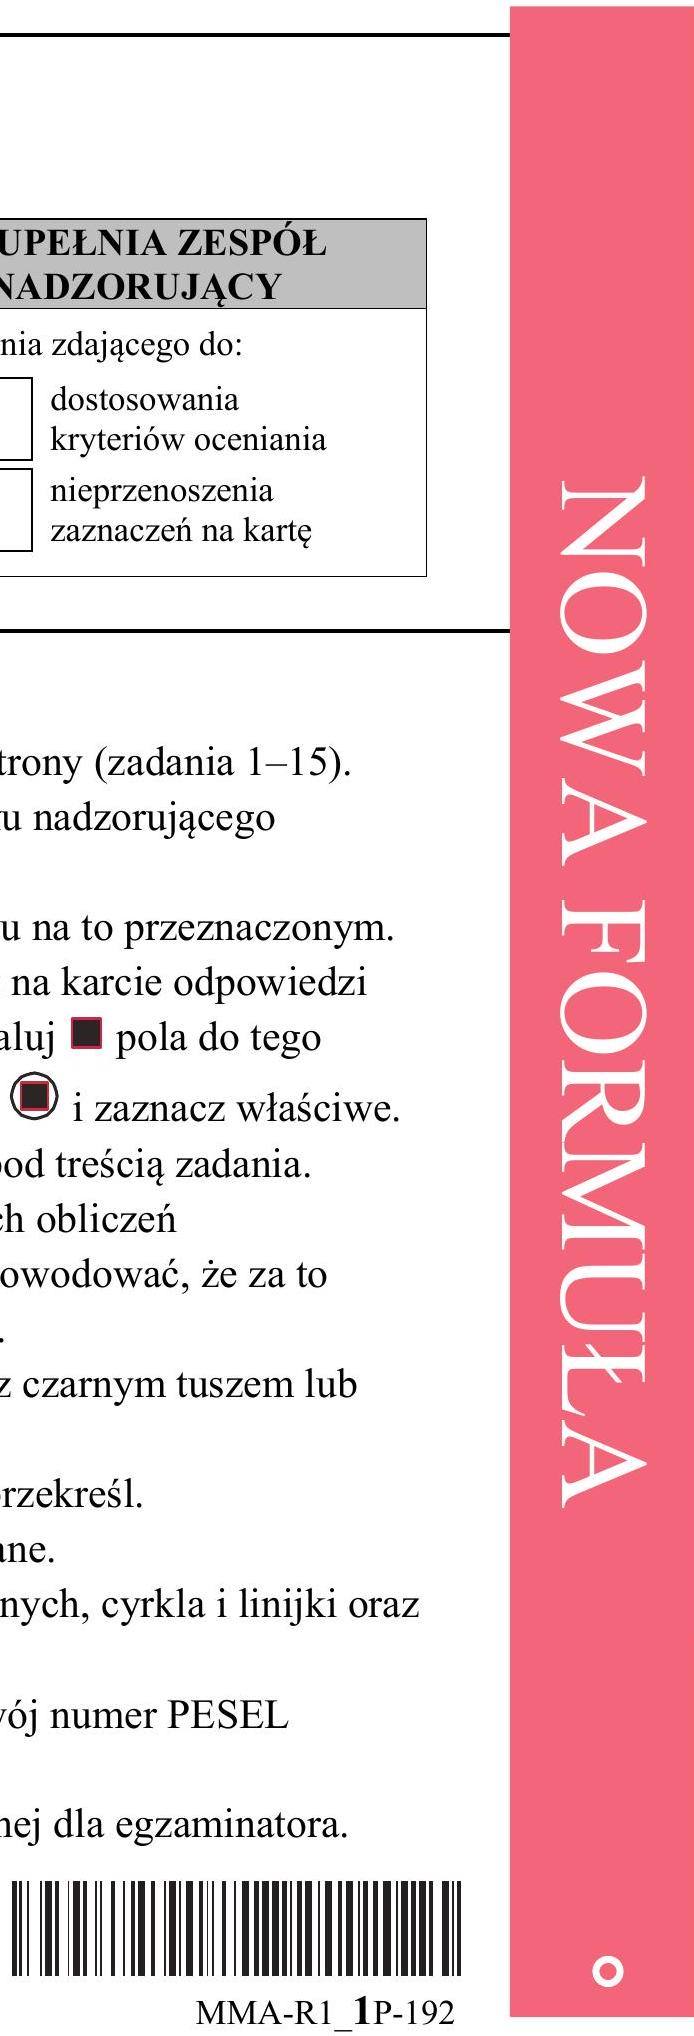
\includegraphics[max width=\textwidth, center]{2024_11_21_9df891ea1c7ef9791261g-01(1)}

W każdym z zadań od 1. do 4. wybierz i zaznacz na karcie odpowiedzi poprawna odpowiedź.

\section*{Zadanie 1. (0-1)}
Dla dowolnych liczb \(x>0, x \neq 1, y>0, y \neq 1\) wartość wyrażenia \(\left(\log _{\frac{1}{x}} y\right) \cdot\left(\log _{\frac{1}{y}} x\right)\) jest równa\\
A. \(x \cdot y\)\\
B. \(\frac{1}{x \cdot y}\)\\
C. -1\\
D. 1

\section*{Zadanie 2. (0-1)}
Liczba \(\cos ^{2} 105^{\circ}-\sin ^{2} 105^{\circ}\) jest równa\\
A. \(-\frac{\sqrt{3}}{2}\)\\
B. \(-\frac{1}{2}\)\\
C. \(\frac{1}{2}\)\\
D. \(\frac{\sqrt{3}}{2}\)

\section*{Zadanie 3. (0-1)}
Na rysunku przedstawiono fragment wykresu funkcji \(y=f(x)\), który jest złożony z dwóch półprostych \(A D\) i \(C E\) oraz dwóch odcinków \(A B\) i \(B C\), gdzie \(A=(-1,0), B=(1,2)\), \(C=(3,0), D=(-4,3), E=(6,3)\).\\
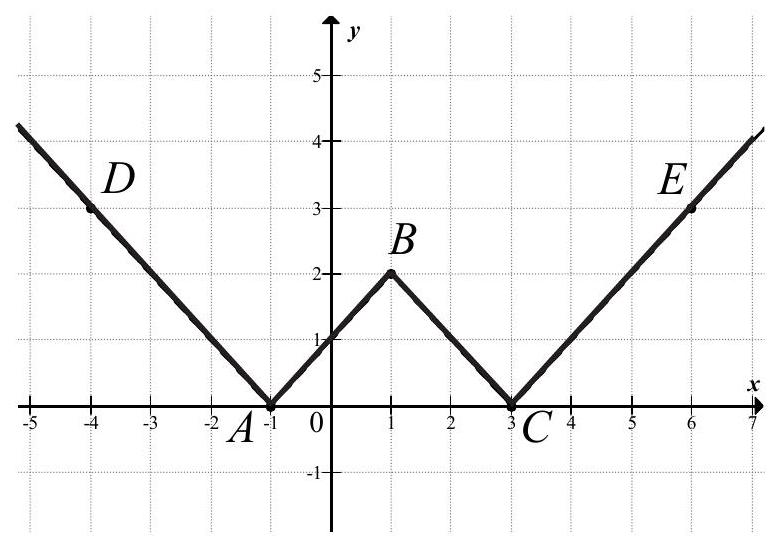
\includegraphics[max width=\textwidth, center]{2024_11_21_9df891ea1c7ef9791261g-02}

Wzór funkcji \(f\) to\\
A. \(f(x)=|x+1|+|x-1|\)\\
B. \(f(x)=||x-1|-2|\)\\
C. \(f(x)=||x-1|+2|\)\\
D. \(f(x)=|x-1|+2\)

\section*{Zadanie 4. (0-1)}
Zdarzenia losowe \(A\) i \(B\) zawarte \(\mathrm{w} \quad \Omega\) są takie, że prawdopodobieństwo \(P\left(B^{\prime}\right)\) zdarzenia \(B^{\prime}\), przeciwnego do zdarzenia \(B\), jest równe \(\frac{1}{4}\). Ponadto prawdopodobieństwo warunkowe \(P(A \mid B)=\frac{1}{5}\). Wynika stąd, że\\
A. \(P(A \cap B)=\frac{1}{20}\)\\
B. \(P(A \cap B)=\frac{4}{15}\)\\
C. \(P(A \cap B)=\frac{3}{20}\)\\
D. \(P(A \cap B)=\frac{4}{5}\)

\section*{BRUDNOPIS}
\begin{center}

\includegraphics[max width=\textwidth]{2024_11_21_9df891ea1c7ef9791261g-03}
\end{center}

\section*{Zadanie 5. (0-2)}
Oblicz granicę

\[
\lim _{n \rightarrow \infty}\left(\frac{9 n^{3}+11 n^{2}}{7 n^{3}+5 n^{2}+3 n+1}-\frac{n^{2}}{3 n^{2}+1}\right)
\]

Wpisz w poniższe kratki - od lewej do prawej - trzy kolejne cyfry po przecinku rozwinięcia dziesiętnego otrzymanego wyniku.\\
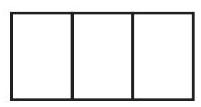
\includegraphics[max width=\textwidth, center]{2024_11_21_9df891ea1c7ef9791261g-04}

\begin{center}
\begin{tabular}{|c|c|c|c|c|c|c|c|c|c|c|c|c|c|c|c|c|c|c|c|c|c|c|c|}
\hline
 &  &  &  &  &  &  &  &  &  &  &  &  &  &  &  &  &  &  &  &  &  &  &  \\
\hline
 &  &  &  &  &  &  &  &  &  &  &  &  &  &  &  &  &  &  &  &  &  &  &  \\
\hline
 &  &  &  &  &  &  &  &  &  &  &  &  &  &  &  &  &  &  &  &  &  &  &  \\
\hline
 &  &  &  &  &  &  &  &  &  &  &  &  &  &  &  &  &  &  &  &  &  &  &  \\
\hline
 &  &  &  &  &  &  &  &  &  &  &  &  &  &  &  &  &  &  &  &  &  &  &  \\
\hline
 &  &  &  &  &  &  &  &  &  &  &  &  &  &  &  &  &  &  &  &  &  &  &  \\
\hline
 &  &  &  &  &  &  &  &  &  &  &  &  &  &  &  &  &  &  &  &  &  &  &  \\
\hline
 &  &  &  &  &  &  &  &  &  &  &  &  &  &  &  &  &  &  &  &  &  &  &  \\
\hline
 &  &  &  &  &  &  &  &  &  &  &  &  &  &  &  &  &  &  &  &  &  &  &  \\
\hline
 &  &  &  &  &  &  &  &  &  &  &  &  &  &  &  &  &  &  &  &  &  &  &  \\
\hline
 &  &  &  &  &  &  &  &  &  &  &  &  &  &  &  &  &  &  &  &  &  &  &  \\
\hline
 &  &  &  &  &  &  &  &  &  &  &  &  &  &  &  &  &  &  &  &  &  &  &  \\
\hline
 &  &  &  &  &  &  &  &  &  &  &  &  &  &  &  &  &  &  &  &  &  &  &  \\
\hline
 &  &  &  &  &  &  &  &  &  &  &  &  &  &  &  &  &  &  &  &  &  &  &  \\
\hline
 &  &  &  &  &  &  &  &  &  &  &  &  &  &  &  &  &  &  &  &  &  &  &  \\
\hline
 &  &  &  &  &  &  &  &  &  &  &  &  &  &  &  &  &  &  &  &  &  &  &  \\
\hline
 &  &  &  &  &  &  &  &  &  &  &  &  &  &  &  &  &  &  &  &  &  &  &  \\
\hline
 &  &  &  &  &  &  &  &  &  &  &  &  &  &  &  &  &  &  &  &  &  &  &  \\
\hline
 &  &  &  &  &  &  &  &  &  &  &  &  &  &  &  &  &  &  &  &  &  &  &  \\
\hline
 &  &  &  &  &  &  &  &  &  &  &  &  &  &  &  &  &  &  &  &  &  &  &  \\
\hline
 &  &  &  &  &  &  &  &  &  &  &  &  &  &  &  &  &  &  &  &  &  &  &  \\
\hline
 &  &  &  &  &  &  &  &  &  &  &  &  &  &  &  &  &  &  &  &  &  &  &  \\
\hline
 &  &  &  &  &  &  &  &  &  &  &  &  &  &  &  &  &  &  &  &  &  &  &  \\
\hline
 &  &  &  &  &  &  &  &  &  &  &  &  &  &  &  &  &  &  &  &  &  &  &  \\
\hline
 &  &  &  &  &  &  &  &  &  &  &  &  &  &  &  &  &  &  &  &  &  &  &  \\
\hline
 &  &  &  &  &  &  &  &  &  &  &  &  &  &  &  &  &  &  &  &  &  &  &  \\
\hline
 &  &  &  &  &  &  &  &  &  &  &  &  &  &  &  &  &  &  &  &  &  &  &  \\
\hline
 &  &  &  &  &  &  &  &  &  &  &  &  &  &  &  &  &  &  &  &  &  &  &  \\
\hline
 &  &  &  &  &  &  &  &  &  &  &  &  &  &  &  &  &  &  &  &  &  &  &  \\
\hline
 &  &  &  &  &  &  &  &  &  &  &  &  &  &  &  &  &  &  &  &  &  &  &  \\
\hline
 &  &  &  &  &  &  &  &  &  &  &  &  &  &  &  &  &  &  &  &  &  &  &  \\
\hline
 &  &  &  &  &  &  &  &  &  &  &  &  &  &  &  &  &  &  &  &  &  &  &  \\
\hline
 &  &  &  &  &  &  &  &  &  &  &  &  &  &  &  &  &  &  &  &  &  &  &  \\
\hline
 &  &  &  &  &  &  &  &  &  &  &  &  &  &  &  &  &  &  &  &  &  &  &  \\
\hline
 &  &  &  &  &  &  &  &  &  &  &  &  &  &  &  &  &  &  &  &  &  &  &  \\
\hline
 &  &  &  &  &  &  &  &  &  &  &  &  &  &  &  &  &  &  &  &  &  &  &  \\
\hline
 &  &  &  &  &  &  &  &  &  &  &  &  &  &  &  &  &  &  &  &  &  &  &  \\
\hline
 &  &  &  &  &  &  &  &  &  &  &  &  &  &  &  &  &  &  &  &  &  &  &  \\
\hline
 &  &  &  &  &  &  &  &  &  &  &  &  &  &  &  &  &  &  &  &  &  &  &  \\
\hline
 &  &  &  &  &  &  &  &  &  &  &  &  &  &  &  &  &  &  &  &  &  &  &  \\
\hline
\end{tabular}
\end{center}

\section*{Zadanie 6. (0-3)}
Rozważamy wszystkie liczby naturalne pięciocyfrowe zapisane przy użyciu cyfr \(1,3,5,7,9\), bez powtarzania jakiejkolwiek cyfry. Oblicz sumę wszystkich takich liczb.\\

\includegraphics[max width=\textwidth, center]{2024_11_21_9df891ea1c7ef9791261g-05}

Odpowiedź: \(\qquad\)

\begin{center}
\begin{tabular}{|c|l|c|c|}
\hline
\multirow{2}{*}{\begin{tabular}{c}
Wypetnia \\
egzaminator \\
\end{tabular}} & Nr zadania & 5. & \(\mathbf{6}\). \\
\cline { 2 - 4 }
 & Maks. liczba pkt & 2 & 3 \\
\cline { 2 - 4 }
 & Uzyskana liczba pkt &  &  \\
\hline
\end{tabular}
\end{center}

\section*{Zadanie 7. (0-2)}
Punkt \(P=(10,2429)\) leży na paraboli o równaniu \(y=2 x^{2}+x+2219\). Prosta o równaniu kierunkowym \(y=a x+b\) jest styczna do tej paraboli w punkcie \(P\). Oblicz współczynnik \(b\).\\

\includegraphics[max width=\textwidth, center]{2024_11_21_9df891ea1c7ef9791261g-06}

Odpowiedź: \(\qquad\)

\section*{Zadanie 8. (0-3)}
Udowodnij, że dla dowolnych dodatnich liczb rzeczywistych \(x\) i \(y\), takich że \(x<y\), i dowolnej dodatniej liczby rzeczywistej \(a\), prawdziwa jest nierówność \(\frac{x+a}{y+a}+\frac{y}{x}>2\).\\

\includegraphics[max width=\textwidth, center]{2024_11_21_9df891ea1c7ef9791261g-07}

\begin{center}
\begin{tabular}{|c|l|c|c|}
\hline
\multirow{2}{*}{\begin{tabular}{c}
Wypetnia \\
egzaminator \\
\end{tabular}} & Nr zadania & 7. & \(\mathbf{8 .}\) \\
\cline { 2 - 4 }
 & Maks. liczba pkt & \(\mathbf{2}\) & \(\mathbf{3}\) \\
\cline { 2 - 4 }
 & Uzyskana liczba pkt &  &  \\
\hline
\end{tabular}
\end{center}

\section*{Zadanie 9. (0-3)}
Dany jest trójkąt równoramienny \(A B C\), w którym \(|A C|=|B C|\). Na ramieniu \(A C\) tego trójkąta wybrano punkt \(M(M \neq A\) i \(M \neq C)\), a na ramieniu \(B C\) wybrano punkt \(N\), w taki sposób, że \(|A M|=|C N|\). Przez punkty \(M\) i \(N\) poprowadzono proste prostopadłe do podstawy \(A B\) tego trójkąta, które wyznaczają na niej punkty \(S\) i \(T\). Udowodnij, że \(|S T|=\frac{1}{2}|A B|\).\\

\includegraphics[max width=\textwidth, center]{2024_11_21_9df891ea1c7ef9791261g-08}\\

\includegraphics[max width=\textwidth, center]{2024_11_21_9df891ea1c7ef9791261g-09}

\begin{center}
\begin{tabular}{|c|l|c|}
\hline
\multirow{2}{*}{\begin{tabular}{l}
Wypelnia \\
egzaminator \\
\end{tabular}} & Nr zadania & 9. \\
\cline { 2 - 3 }
 & Maks. liczba pkt & \(\mathbf{3}\) \\
\cline { 2 - 3 }
 & Uzyskana liczba pkt &  \\
\hline
\end{tabular}
\end{center}

\section*{Zadanie 10. (0-4)}
Punkt \(D\) leży na boku \(A B\) trójkąta \(A B C\) oraz \(|A C|=16,|A D|=6,|C D|=14\) i \(|B C|=|B D|\). Oblicz obwód trójkąta \(A B C\).\\

\includegraphics[max width=\textwidth, center]{2024_11_21_9df891ea1c7ef9791261g-10}\\

\includegraphics[max width=\textwidth, center]{2024_11_21_9df891ea1c7ef9791261g-11}

Odpowiedź: \(\qquad\)

\begin{center}
\begin{tabular}{|c|l|c|}
\hline
\multirow{2}{*}{\begin{tabular}{l}
Wypelnia \\
egzaminator \\
\end{tabular}} & Nr zadania & 10. \\
\cline { 2 - 3 }
 & Maks. liczba pkt & 4 \\
\cline { 2 - 3 }
 & Uzyskana liczba pkt &  \\
\hline
\end{tabular}
\end{center}

\section*{Zadanie 11. (0-6)}
Dane są okręgi o równaniach \(x^{2}+y^{2}-12 x-8 y+43=0\) i \(x^{2}+y^{2}-2 a x+4 y+a^{2}-77=0\). Wyznacz wszystkie wartości parametru \(a\), dla których te okręgi mają dokładnie jeden punkt wspólny. Rozważ wszystkie przypadki.\\

\includegraphics[max width=\textwidth, center]{2024_11_21_9df891ea1c7ef9791261g-12}\\

\includegraphics[max width=\textwidth, center]{2024_11_21_9df891ea1c7ef9791261g-13}

Odpowiedź: \(\qquad\)

\begin{center}
\begin{tabular}{|c|l|c|}
\hline
\multirow{2}{*}{\begin{tabular}{l}
Wypelnia \\
egzaminator \\
\end{tabular}} & Nr zadania & 11. \\
\cline { 2 - 3 }
 & Maks. liczba pkt & 6 \\
\cline { 2 - 3 }
 & Uzyskana liczba pkt &  \\
\hline
\end{tabular}
\end{center}

\section*{Zadanie 12. (0-6)}
Trzywyrazowy ciąg \((a, b, c)\) o wyrazach dodatnich jest arytmetyczny, natomiast ciąg \(\left(\frac{1}{a}, \frac{2}{3 b}, \frac{1}{2 a+2 b+c}\right)\) jest geometryczny. Oblicz iloraz ciągu geometrycznego.\\

\includegraphics[max width=\textwidth, center]{2024_11_21_9df891ea1c7ef9791261g-14}\\

\includegraphics[max width=\textwidth, center]{2024_11_21_9df891ea1c7ef9791261g-15}

Odpowiedź:

\begin{center}
\begin{tabular}{|c|l|c|}
\hline
\multirow{2}{*}{\begin{tabular}{l}
Wypelnia \\
egzaminator \\
\end{tabular}} & Nr zadania & 12. \\
\cline { 2 - 3 }
 & Maks. liczba pkt & 6 \\
\cline { 2 - 3 }
 & Uzyskana liczba pkt &  \\
\hline
\end{tabular}
\end{center}

Zadanie 13. (0-6)\\
Wielomian określony wzorem \(W(x)=2 x^{3}+\left(m^{3}+2\right) x^{2}-11 x-2(2 m+1)\) jest podzielny przez dwumian \((x-2)\) oraz przy dzieleniu przez dwumian \((x+1)\) daje resztę 6 . Oblicz \(m\) i dla wyznaczonej wartości \(m\) rozwiąż nierówność \(W(x) \leq 0\).\\

\includegraphics[max width=\textwidth, center]{2024_11_21_9df891ea1c7ef9791261g-16}\\

\includegraphics[max width=\textwidth, center]{2024_11_21_9df891ea1c7ef9791261g-17}

Odpowiedź: \(\qquad\)

\begin{center}
\begin{tabular}{|c|l|c|}
\hline
\multirow{2}{*}{\begin{tabular}{c}
Wypelnia \\
egzaminator \\
\end{tabular}} & Nr zadania & 13. \\
\cline { 2 - 3 }
 & Maks. liczba pkt & 6 \\
\cline { 2 - 3 }
 & Uzyskana liczba pkt &  \\
\hline
\end{tabular}
\end{center}

\section*{Zadanie 14. (0-4)}
Rozwiąż równanie \((\cos x)\left[\sin \left(x-\frac{\pi}{3}\right)+\sin \left(x+\frac{\pi}{3}\right)\right]=\frac{1}{2} \sin x\).\\
\(\qquad\)\\

\includegraphics[max width=\textwidth, center]{2024_11_21_9df891ea1c7ef9791261g-19}

Odpowiedź: \(\qquad\)

\begin{center}
\begin{tabular}{|c|l|c|}
\hline
\multirow{2}{*}{\begin{tabular}{l}
Wypelnia \\
egzaminator \\
\end{tabular}} & Nr zadania & 14. \\
\cline { 2 - 3 }
 & Maks. liczba pkt & 4 \\
\cline { 2 - 3 }
 & Uzyskana liczba pkt &  \\
\hline
\end{tabular}
\end{center}

\section*{Zadanie 15. (0-7)}
Rozważmy wszystkie graniastosłupy prawidłowe trójkątne o objętości \(V=2\). Wyznacz długości krawędzi tego z rozważanych graniastosłupów, którego pole powierzchni całkowitej jest najmniejsze. Oblicz to najmniejsze pole.\\

\includegraphics[max width=\textwidth, center]{2024_11_21_9df891ea1c7ef9791261g-20}\\

\includegraphics[max width=\textwidth, center]{2024_11_21_9df891ea1c7ef9791261g-21}

Odpowiedź: \(\qquad\)

\begin{center}
\begin{tabular}{|c|l|c|}
\hline
\multirow{2}{*}{\begin{tabular}{l}
Wypelnia \\
egzaminator \\
\end{tabular}} & Nr zadania & 15. \\
\cline { 2 - 3 }
 & Maks. liczba pkt & 7 \\
\cline { 2 - 3 }
 & Uzyskana liczba pkt &  \\
\hline
\end{tabular}
\end{center}

\section*{BRUDNOPIS (nie podlega ocenie)}

\end{document}